\documentclass{ximera}

\newcommand{\RR}{\mathbb R}
\renewcommand{\d}{\,d}
\newcommand{\dd}[2][]{\frac{d #1}{d #2}}
\renewcommand{\l}{\ell}
\newcommand{\ddx}{\frac{d}{dx}}
\newcommand{\dfn}{\textbf}
\newcommand{\eval}[1]{\bigg[ #1 \bigg]}


\author{Jim Talamo}
\license{Creative Commons 3.0 By-bC}


\outcome{}


\begin{document}
\begin{exercise}
There are many different tests that can be used to test whether a given series converges or diverges.  As a result, it is important to develop a good sense for quickly narrowing down which tests make sense to apply to a given series just by inspecting the given series.  A fundamentally important fact allows us to gain some insight into the Root Test:

\begin{fact}
Let $p(x)$ be a polynomial.  Then:

\[
\lim_{n \to \infty} \sqrt[n]{p(n)} = 1.
\]
\end{fact}

\begin{exercise}
To gain a little practice, suppose that $p(x) = x^5$.  Then the limit to evaluate is:

\[
\lim_{n \to \infty}\sqrt[n]{p(n)} = \sqrt[n]{\answer{n^5}}
\]

Taking $n \to \infty$ gives the indeterminate form $\answer{\infty}^{\answer{0}}$. 
(Use $\infty$ or $-\infty$ where appropriate)

As such, we can use logarithms to convert this to a more manageable form.

Set $L = \lim_{n \to \infty} \sqrt[n]{a_n}$.  Taking the logarithm of both sides gives:

\[
\ln L = \ln  \left( \lim_{n \to \infty} \left(n^5\right)^{1/n} \right) = \lim_{n \to \infty} \ln \left(n^5\right)^{1/n} 
\]

Using the properties of logarithms:
\[
\ln L = \lim_{n \to \infty} \answer{\frac{1}{n}} \ln \left(n^5\right) = \lim_{n \to \infty} \answer{\frac{5}{n}} \ln(n)
\]

This limit has indeterminate form $0 \cdot \infty$. This is easy to convert; indeed:
\[
\ln L = \lim_{n \to \infty} \answer{\frac{5}{n}} \ln(n) = \lim_{n \to \infty} \answer{\frac{5\ln(n)}{n}}
\]

\begin{exercise}
By growth rates: 

\[
\ln L  = \lim_{n \to \infty} \frac{5\ln(n)}{n} = \answer{0}
\]

Hence, $L = \answer{1}$.
\end{exercise}

Note that had we used a higher degree than $5$ in the preceding argument, it would not affect the conclusion; indeed, if we perform the same argument for $x^m$ for $m>0$, the eventual limit to compute in the above argument would be:

\[
\ln L  = \lim_{n \to \infty} \frac{m\ln(n)}{n} = \answer{0}
\] 


\begin{exercise}
To explore this a little more, now set $p(x) = x^5+4x^3+7$.  Then:
\[
\lim_{n \to \infty}\sqrt[n]{p(n)} = \lim_{n \to \infty} \sqrt[n]{\answer{n^5+4n^3+7}}
\]

We can do some algebra:

\[
\sqrt[n]{n^5+4n^3+7} = \sqrt[n]{n^5} \cdot \sqrt[n]{\answer{1+\frac{4}{n^2}+\frac{7}{n^5}}}
\]

\begin{exercise}
Thus, we can write:

\[
\lim_{n \to \infty}\sqrt[n]{p(n)} = \lim_{n \to \infty} \sqrt[n]{n^5} \cdot \left(1+\frac{4}{n^2}+\frac{7}{n^5}\right)^{1/n}
\]

Notice that as $n \to \infty$, the second multiple has the form $\answer{1}^{\answer{0}}$, which is not an indeterminate form!  Hence, $\lim_{n \to \infty}  \left(1+\frac{4}{n^2}+\frac{7}{n^5}\right)^{1/n} = \answer{1}$, and:

\begin{image}
  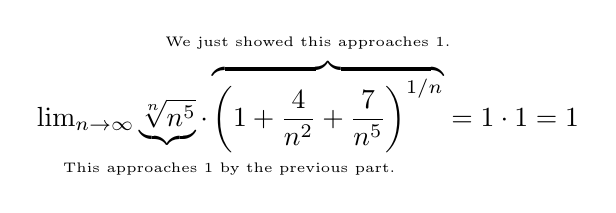
\begin{tikzpicture}
        \node at (0,0) {
          $\lim_{n \to \infty}  \underbrace{\sqrt[n]{n^5}} \cdot \overbrace{\left(1+\frac{4}{n^2}+\frac{7}{n^5}\right)^{1/n}}=1 \cdot 1 = 1$
        };
        \node at (0,.8)  {\tiny{We just showed this approaches $1$.}};
        \node at (-1,-.8) {\tiny{This approaches $1$ by the previous part.}};
      \end{tikzpicture}
  \end{image}


\end{exercise}

\end{exercise}


\begin{exercise}
One of the major consequences of this is that multiplying or dividing a given \emph{sequence} by a polynomial will not affect the limit required in the Root Test.  Indeed, consider the series $\sum_{k=1}^{\infty} \frac{1}{2^k}$.  Note that this is a geometric series, but we could establish its convergence using the Root Test.  Indeed, here:

\[
L = \lim_{n \to \infty} \sqrt[n]{a_n} = \lim_{n \to \infty}\sqrt[n]{\frac{1}{2^n}} = \answer{\frac{1}{2}}
\]

Now, let's multiply the original sequence defined by the rule $a_n = \left(\frac{1}{2}\right)^n$ by the polynomial $p(n) = n^5$ and try to sum its terms.  That is, we want to consider the series $\sum_{k=1}^{\infty} \frac{k^5}{2^k}$. We find:

\[
L =  \lim_{n \to \infty} \sqrt[n]{\frac{n^5}{2^n}} =  \lim_{n \to \infty} \frac{\sqrt[n]{n^5}}{\sqrt[n]{2^n}}  =  \lim_{n \to \infty} \frac{\sqrt[n]{n^5}}{\answer{2}} = \answer{\frac{1}{2}}
\]

Introducing the $n^5$ term into the numerator did not affect the value of $L$.

Indeed, for the series $\sum_{k=1}^{\infty} \frac{1}{2^k}$, we found that $L=\answer{\frac{1}{2}}$ and for the series $\sum_{k=1}^{\infty} \frac{k^5}{2^k}$, we found $L=\answer{\frac{1}{2}}$. 

\begin{exercise}
One of the major consequences of this now is that a series must have a term that grows at least exponentially in order for the Root Test to have a chance to be conclusive!  More explicitly, let $p, q > 0$, $a>1$, and consider the growth rates results for \emph{sequences}:

\begin{image}
  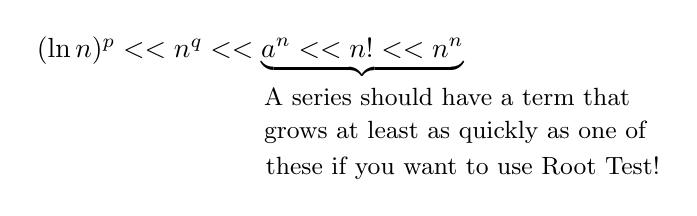
\begin{tikzpicture}
        \node at (0,0) {
          $(\ln n)^p << n^q << \underbrace{a^n << n! << n^n}$
        };
        \node at (2.5,-.5) {\small{A series should have a term that}};
         \node at (2.6,-.95) {\small{grows at least as quickly as one of}};
         \node at (2.7,-1.4) {\small{these if you want to use Root Test! }};
      \end{tikzpicture}
  \end{image}

Without performing any calculations, determine which of the following series would the Root Test would be conclusive.  That is, which of the following would either converge or diverge as a consequence of the Root Test?
\begin{selectAll}
\choice{$\sum_{k=1}^{\infty} \frac{k^3+2k-1}{k^2+2}$}
\choice[correct]{$\sum_{k=1}^{\infty} \left(\frac{\ln(k) +k^2}{k+4}\right)^k$}
\choice[correct]{$\sum_{k=1}^{\infty} \frac{k^{10}}{5^k}$}
\choice{$\sum_{k=1}^{\infty} \frac{(\ln k)^{80}}{k^5}$}
\choice{$\sum_{k=1}^{\infty} k^{2018}$}
\choice[correct]{$\sum_{k=1}^{\infty} \frac{2^k}{k^k}$}
\end{selectAll}

\end{exercise}
\end{exercise}
\end{exercise}
\end{exercise}
\end{document}
